%TODO The caption and the image are from http://swarmlab.unimaas.nl/stico/stico-principle/ so there needs to be a reference to here

One way of covering the entire area of the environment is to try to equally disperse the guards over the area in a way that tries to cover as much of the area as possible. An algorithm that attempts to do this is the so called StiCo algorithm. In the StiCo algorithm all agents lay down a pheromone trail that other agents can detect. The principle is that once an agent detects a pheromone it changes its direction so to not cover an area that another agent already covers. In an non-open environment also the walls and other obstructions can be seen as these pheromones. In nature the pheromones are scents. In our world, the pheromones will be beacons dropped by the agent which can be seen by other agents \cite{ranjbar2012multi}.

The StiCo algorithm needs a base movement from which to start. This base movement is moving at a constant forward and angular velocity, which results into describing a circle (if not obstructed). Any time the agent encounters a pheromone trail, it simply changes its angular velocity to move another direction. To determine what direction is the best one to avoid the pheromone trail the agent has two different sensors: an interior, and an exterior. The interior sensor is the one on the inside of the circular motion, and the exterior one is the one on the outside of the circular motion described by the agent. If the interior sensor picks up the pheromone trail, the easiest way to avoid the pheromones is to invert the angular velocity. If the exterior sensor picks up the pheromone trail the agent should temporarily increase its angular velocity to avoid the pheromone trail (see alg.~7, fig. \ref{fig:movingDirections})~\cite{ranjbar2012multi}.

\begin{algorithm}
\label{alg:StiCo}
\caption{Iteration of the StiCo Algorithm~\protect\cite{ranjbar2012multi}}
	\While{no pheromone encountered}{
		Move with velocity $v$ and angular velocity $a$\;
	}
	\eIf{Encountered pheromone at interior sensor}{
		$a\leftarrow -a$\;
	}{
		\While{Pheromone is detected}{
			increase $a$\;
		}
		Set $a$ back to the original value\;
	}
\end{algorithm}

\begin{figure}
\centering
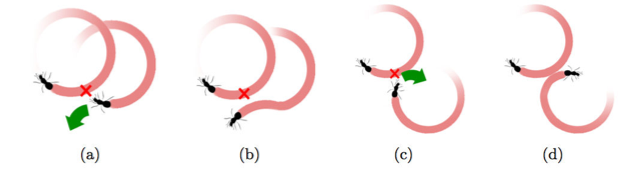
\includegraphics[width=\columnwidth]{images/stico.png}
\caption{StiCo coordination principle (a) and (c) before pheromone detection (b) and (d) after pheromone detection~\protect\cite{ranjbar2012multi}}
\label{fig:movingDirections}
\end{figure}

A great advantage of the StiCo algorithm, apart from its simplicity, is that no prior map of the environment is needed. Therefore, the entire exploration phase can be skipped and not bother with trying to figure out when exactly an agent should explore the environment, and when it should cover the known map. Also there is no initial time the agent needs to spend exploring.

The other side of the coin is that the agent also does not use a map of the environment. It does not intelligently cope with features of the environment such as entries, doors, windows, exits, sentry towers, etc.

Moreover, the algorithm often reaches an equilibrium, namely when no territories, the area described by the circular motion of an agent, of the agents intersect. There, however, is no guarantee that this equilibrium covers the entire area. One could argue that if this is the case, there are simply not a sufficient amount of guards guarding the premise, but it is quite obvious that in a mansion with only one guard, the guard should not just stand in the main hall walking circles, hoping to run into an intruder.

% the source of this text is http://swarmlab.unimaas.nl/stico/stico-principle/